\subsection{Gliederung der Arbeit}
\label{sub:gliederung_der_arbeit}
  Das Projekt wurde nach dem Design-Prinzip \texttt{"`The Double Diamond"'}\footnote{\url{http://www.designcouncil.org.uk/news-opinion/design-process-what-double-diamond}} bearbeitet, welcher der vorliegenden schriftlichen Ausarbeitung auch als Gliederungsgrundlage dient. Der Double Diamond wurde vom British Design Council 2005 entwickelt und soll im Folgenden kurz beschrieben werden.\parencite{designcouncil}

  \begin{figure}[htbp]
    \begin{center}
      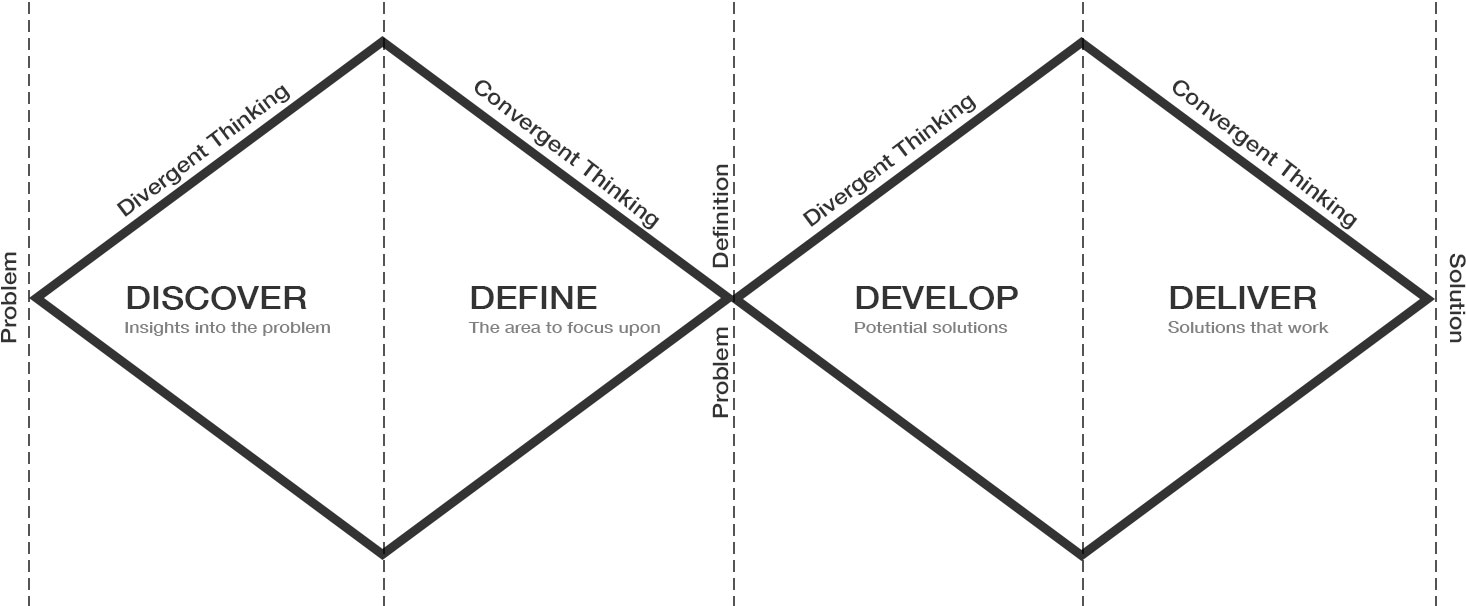
\includegraphics[width=0.9\textwidth]{double_diamond}
      \caption{"`The Double Diamond"' eigene Abbildung nach \parencite{designcouncil}}
      \label{fig:double_diamond}
    \end{center}
  \end{figure}

  Der Double Diamond beschreibt einen iterativen Prozess. Wie in allen kreativen Prozessen werden dabei eine Reihe von möglichen Ideen geschaffen ("divergentes Denken"), bevor sie verfeinert und auf die beste Idee reduziert werden ("konvergentes Denken"). Der Double Diamond zeigt jedoch an, dass dies zweimal geschieht - einmal zur Bestätigung der Problemdefinition und einmal zur Erstellung der Problemlösung. Einer der größten Fehler wäre es, den linken Diamanten und damit auch die Zieldimension zu vernachlässigen und am Ende womöglich das falsche Problem zu lösen.

  \begin{itemize}[label={}]
    \item \textbf{Discover:} Der erste Teil des Double Diamond steht am Anfang des Projektes. Hier wird versucht, die Welt neu zu sehen, Neues wahrzunehmen und Einsichten in das zu lösende Problem zu sammeln.

    \item \textbf{Define:} Der zweite Teil stellt die Definitionsphase dar. Dabei wird versucht, alle in der Entdeckungsphase identifizierten Möglichkeiten zu verstehen. Ziel ist es, ein klares Briefing zu entwickeln, das die grundsätzlichen Herausforderungen umreißt.

    \item \textbf{Develop:} Der dritte Teil markiert eine Entwicklungsphase, in der Lösungen oder Konzepte erstellt, prototypisiert, getestet und iteriert werden. Dieser Prozess des Ausprobierens hilft, Ideen zu verbessern und zu verfeinern.

    \item \textbf{Deliver:} Der letzte Teil des Double Diamond ist die Lieferphase, in der das daraus resultierende Projekt (z. B. ein Produkt, eine Dienstleistung oder eine Umwelt) abgeschlossen, produziert und in Betrieb genommen wird.

  Auf den Aufbau dieser Arbeit bezogen, werden diese Phasen auch für die Bezeichnung der Kapitel verwendet, in denen der Entwicklungsprozess der Webanwendung beschrieben wird. 

  \end{itemize}

% sub:gliederung_der_arbeit (end)